\documentclass[]{thesis-ekf}
\usepackage[T1]{fontenc}
\PassOptionsToPackage{defaults=hu-min}{magyar.ldf}
\usepackage[magyar]{babel}
\usepackage{mathtools,amssymb,amsthm,pdfpages}
\footnotestyle{rule=fourth}


\usepackage{longtable}
\usepackage{array}
\usepackage{hyperref}
\usepackage{media9}
\usepackage{xcolor}
\usepackage{listings}

\begin{document}
	
	\institute{Matematikai és Informatikai Intézet}
	\title{Python alapú grafikus alkalmazásfejlesztés}
	\author{Mészáros Réka\\Programtervező informatikus BSc}
	\supervisor{Kovács Ádám\\Tanársegéd}
	\city{Eger}
	\date{2026}
	\maketitle
	
	\tableofcontents
	\listoffigures 
	
	\lstdefinestyle{pythonstyle}{
		language=Python, 
		backgroundcolor=\color{gray!10},
		keywordstyle=\bfseries\color{blue},
		commentstyle=\itshape\color{green!50!black},
		stringstyle=\color{red!60!black},
		showstringspaces=false,
		numbers=left,
		numberstyle=\tiny\color{gray},
		frame=single,
		breaklines=true,
		captionpos=b
	}
	
	
	\chapter{Bevezetés}
	
	\section{Témaválasztás}
	
	Az elmúlt években egyre nagyobb hangsúlyt kaptak az interaktív, digitális tanulási eszközök, különösen a vizuális szemléltetést igénylő tantárgyakban. A hagyományos oktatási módszerek mellett egyre fontosabbá váltak azok a szoftveres megoldások, amelyek játékos módon támogatják a tanulók ismeretszerzését. Ez különösen igaz a természettudományos tantárgyakra, ahol az elméleti ismeretek megértését jelentősen segítheti a vizuális szemléltetés.
	
	
	A kémia oktatásában a kísérletek és reakciók vizuális megfigyelése és kipróbálása kifejezetten fontos, hiszen ezek segítségével a tanulók könnyebben megérthetik az egyes anyagok tulajdonságait. Ugyanakkor az iskolai laboratóriumi környezet sok esetben korlátozott lehet. Az eszközök hiánya, a veszélyes anyagok használata, vagy az idő- és költségigény gyakran megnehezíti a gyakorlati oktatást.
	
	Általános iskolai és gimnáziumi tanulmányaim során azt tapasztaltam, hogy a laboratóriumi környezetet elsősorban a természettudományos irányba továbbtanuló diákok használták rendszeresen. Azonban ha kísérletezésre került sor az óra keretein belül, az jelentős felkészülést és időt vett el a tanórából. Ekkor értettem  meg igazán miért is az elméleti oktatásra fókuszálnak a pedagógusok. 
	
	\section{Téma bemutatása}
	
	A szakdolgozat célja egy olyan oktatási célú játékalkalmazás fejlesztése, amely virtuális laboratóriumi	környezetben támogatja kémiai reakciók gyakorlását.
	Az alkalmazás elsődleges célja, hogy támogassa a tanulók kémiai ismereteinek elmélyítését, valamint játékos formában segítse az összefüggések megértését.Emellett fontos cél volt, hogy a diákok tanári segítség nélkül is gyakorolhassák az órán tanult vegyületek előállításának lépéseit.
	
	A program lehetőséget biztosít különböző anyagok és eszközök kiválasztására, játékmezőre helyezésére	és a reakciók automatikus felismerésére.
	
	Az alkalmazás egyik fontos funkciója a keresőrendszer, amely támogatja a felhasználót egy adott anyag	előállítási lépéseinek megtalálásában. Ez különösen hasznos lehet a tanulási folyamat során, mivel lépésről lépésre bemutatja az adott reakcióhoz vezető műveletsort.
	
	A dolgozat során bemutatom a fejlesztéshez használt technológiákat, a rendszertervet, az adatbázis felépítését, valamint az alkalmazás megvalósításának folyamatát. Emellett részletesen ismertetem a program működését, a főbb modulokat és azok kapcsolatát.
	
	A témaválasztásomat elsősorban az oktatás és az informatika összekapcsolásának lehetősége motiválta. A kémiai reakciók összeállításában szakmai segítséget kaptam, amely hozzájárult a példák kiválasztásához.
	
	Véleményem szerint a modern oktatásban egyre nagyobb szerepet kapnak a digitális eszközök, különösen azok az interaktív alkalmazások, amelyek képesek a tanulási folyamatot szemléletesebbé és élményszerűbbé tenni.
	
	A kémia tantárgy sajátossága, hogy az elméleti ismeretek mellett fontos szerepet kap a gyakorlati megvalósítás. Sok tanuló számára hatékonyabb lehet, ha az elméleti reakciókat vizuálisan és interaktívan is megfigyelheti A laboratóriumi kísérletek segítik a tanulókat abban, hogy jobban megértsék az anyagok tulajdonságait, valamint a különböző reakciók sorrendjét. Ugyanakkor a valós laboratóriumi környezet használata sok esetben korlátozott, mivel speciális eszközöket, anyagokat és biztonságos körülményeket igényel.
	
	A virtuális laboratóriumi környezet azért hasznos, mert veszélytelen és költséghatékony gyakorlási lehetőséget biztosít. Ezen kívül a játékos megközelítés motiváló hatással lehet a diákokra, különösen a fiatalabb korosztály számára.
	
	\section{Hasonló alkalmazások}
	
	\chapter{Technológiai áttekintés} 
	\section{Programozási nyelvek}
	
	\subsection{Python}
	
	A Python\cite{Python} egy magas szintű objektumorientált programozási nyelv, amelyet Guido van Rossum fejlesztett ki az 1980-as évek végén. A fejlesztést az ABC programozási nyelv utódjaként kezdte meg. Első megjelenése 1991-ben történt. Előtérbe helyezi a kód olvashatóságát, egyszerűségét és a vele való munka megkönnyítését. Szintaxisa letisztult, könnyen érthető.
	
	A Python széles körben használt nyelv többek között adatfeldolgozásban, gépi tanulásban,	webfejlesztésben és oktatási célú alkalmazások készítésében.
	
	Tanulmányaim során több programozási nyelvvel is megismerkedtem, ilyenek például a C++\cite{C++}, C-Sharp\cite{C-Sharp} vagy Java\cite{Java}, a projekt megvalósításához azonban a Python mellett döntöttem.
	
	\textbf{Python előnyei:}
	\begin{itemize}
		\item \textbf{Egyszerű szintaxis:} A Python kódja könnyen olvasható és érthető, ami megkönnyíti a vele való munkát.
		\item \textbf{Gyors fejlesztés:} A dinamikus típusrendszer lehetővé teszi, hogy a változók típusait nem szükséges előre deklarálni.
		\item \textbf{Gazdag könyvtárkészlet:} A Pythonhoz számos, különböző feladatokra használható könyvtár érhető el.
		\item \textbf{Keresztplatformosság:} A Python programok Windows, Linux és macOS rendszereken azonos módon futtathatóak.
		\item \textbf{Oktatási célokra alkalmas:} A Python széles körben használt oktatási nyelvként, amely ezáltal ideális egy  célú alkalmazáshoz.
	\end{itemize}
	
	\textbf{Korlátai}
	\begin{itemize}
		\item \textbf{Teljesítmény:} A Python lassabb, mint a fordított nyelvek (C++, Java), de az oktatási alkalmazásokhoz elegendő.
		\item \textbf{Memória-felhasználás:} a runtime nagyobb memóriát igényel, mint az alacsonyabb szintű nyelvek.
		\item \textbf{Telepítési követelmények:} Szükséges a Python futtatókörnyezet telepítése.
	\end{itemize}
	
	\subsection{SQL}
	
	A Structured Query Language (röviden SQL\cite{SQL}) az IBM-nél indult fejlesztésként jelent meg az 1970-es években, és relációs adatbázisok kezelésére szolgál. Főbb lehetőségei a lekérdezés, módosítás, törlés illetve adatbázis létrehozása és kezelése.
	
	A projektben MySQL-t használtam, mert alkalmas a reakciók, anyagok és eszközök strukturált tárolására
	
	\section{GitHub}
	
	A GitHub\cite{GitHub} egy webalapú platform, szolgáltatás mely a Git\cite{Git} verziókezelő rendszerre épül. Fontos szerepet játszik a kód online tárolásában és elérhetőségében. Lehetőséget ad több fejlesztő együttműködésére és a kód verziókezelésére.
	
	A fejlesztést lokálisan végeztem, GitHubot pedig elsősorban a forráskód publikálására és beadási elérhetővé tételére használtam.
	
	\textbf{A Git lehetővé teszi:}
	\begin{itemize}
		\item A kód változásainak követését (commit history).
		\item Az előző verziókhoz való visszatérést (checkout).
		\item A verziókezelés helyi biztonsági mentésként is hasznos lehet, és segíti a korábbi állapotok visszakeresését.
		
	\end{itemize}
	
	A projekt publikálásához a GitHub platformot használtam, amely a következő előnyöket biztosítja:
	\begin{itemize}
		\item \textbf{Nyílt forráskód:} Az alkalmazás forráskódja publikusan elérhető a GitHub repository-ban, amely megkönnyíti az oktatási célú felhasználást.
		\item \textbf{Dokumentáció:} Minden fontos információ, például telepítési útmutató, megtalálható.
		\item \textbf{Hozzáférhetőség:} A tanárok és diákok bármikor letölthetik és futtathatják az alkalmazást saját gépükön.
		\item \textbf{Közösségi visszajelzés:} Az Issues funkcióval felhasználók jelezhetik a hibákat vagy javaslatokat tehetnek a program bővítésére.
	\end{itemize}
	
	\section{Fejlesztői környezetek}
	\subsection{PyCharm}
	
	A projekt megvalósítása során elsődleges fejlesztői környezetként a \textbf{PyCharm}\cite{PyCharm} integrált fejlesztői környezetet (IDE) alkalmaztam, amelyet a JetBrains fejlesztett kifejezetten Python alapú projektekhez. A választás egyik fő oka ismét gimnáziumi éveimbe nyúlik vissza, ahol megismertem a fejlesztőkörnyezetet és megszerettem.
	
	A PyCharm számos olyan funkciót biztosít, amely jelentősen megkönnyítette a fejlesztési folyamatot. Ezek közé tartozik a szintaxiskiemelés, a hibák valós idejű jelzése, valamint a refaktorálási lehetőségek. Ezek az eszközök hozzájárultak a kód olvashatóságának javításához és a hibák számának csökkentéséhez.
	
	A grafikus alkalmazás fejlesztése szempontjából külön előnyt jelentett, hogy a PyCharm jól támogatta a PyGame\cite{PyGame} könyvtár használatát, valamint megkönnyítette a moduláris projektstruktúra kezelését.
	
	\subsection{Visual Studio Code}
	
	A Visual Studio Code (röviden VS Code)\cite{VisualStudioCode} egy, a Microsoft által fejlesztett, ingyenes és nyílt forráskódú kódszerkesztő. Első verziója 2015-ben jelent meg, azóta az egyik legismertebb fejlesztői eszközzé vált.
	
	Számomra legfőbb előnye széles körű bővítményválasztéka. Fontos tulajdonsága az is, hogy több, különböző fájlt is képes kezelni, ilyenek például a .tex, .py, .txt.
	
	Integrálja a Git verziókezelést, azáltal támogatva a projektek fejlesztését.
	
	A VS Code Windows, Linux és macOS rendszereken is használható, ami megkönnyíti a többplatformos fejlesztést.
	
	\subsection{PhPMyAdmin}
	
	A phpMyAdmin\cite{phpMyAdmin} egy ingyenes, webalapú adatbázis-kezelő eszköz, amelyet PHP nyelven fejlesztettek ki. Elsősorban a MySQL adatbázisok grafikus kezelésére szolgál.
	
	Grafikus megjelenése miatt elősegíti az adatbázisok vizuális megjelenését és azok módosításait. Alapszintű műveletek grafikus felületen is elvégezhetők, ugyanakkor az adatbázis helyes tervezéséhez és ellenőrzéséhez SQL-ismeret szükséges.
	
	Böngészőben futtatható felület, amely a háttérben egy MySQL szerverként dolgozik, XAMPP\cite{Apache} rendszerekben elterjedt.
	
	\subsection{Elérhetőségi linkek}
	
	A projekt elérhetőségét az alábbi helyen biztosítom:
	
	GitHub repository: \url{https://github.com/MRekaa/szakdolgozat} 
	
	\section{Használt csomagok} 
	
	\subsection{Pygame könyvtár}
	
	A grafikus megjelenítés és a felhasználói interakciók megvalósításához a Pygame\cite{PyGame2} könyvtárat használtam. A Pygame egy Python alapú, nyílt forráskódú fejlesztői könyvtár, amelyet főként 2D-s játékok és grafikus alkalmazások készítésére használnak.
	
	A könyvtár a \textit{Simple DirectMedia Layer (SDL)}\cite{SDL} multimédiás keretrendszerre épül, amely stabil alapot biztosít a grafikai megjelenítéshez, az eseménykezeléshez, valamint a hang- és képfeldolgozáshoz. Ennek köszönhetően a Pygame széles körben alkalmazható interaktív alkalmazások fejlesztésére.
	
	A szakdolgozat fejlesztése során a Pygame megfelelő választásnak bizonyult, mivel lehetővé tette a 2D-s játékmező egyszerű és hatékony megvalósítását, az objektumok megjelenítését, a sprite-ok megjelenítését valamint a drag-and-drop jellegű felhasználói interakciók kezelését.
	
	
	\textbf{PyGame tulajdonságai}
	\begin{itemize}
		\item \textbf{Keresztplatformosság:} A Pygame támogatja a Windows, Linux és macOS operációs rendszereket, így az alkalmazás különböző környezetekben is futtatható.
		
		\item \textbf{Széles körű támogatás:} Nagy fejlesztői közösséggel rendelkezik, ezért számos dokumentáció, útmutató és oktatóanyag érhető el hozzá.
		
		\item \textbf{Játékfejlesztési funkciók:} A Pygame támogatja a sprite-kezelést, ütközésvizsgálatot és eseménykezelést, amelyek elengedhetetlenek voltak a projekt megvalósításához.
	\end{itemize}
	
	\subsection{MySQL-connector-python}
	
	Az adatbázis-kapcsolat kezeléséhez a mysql-connector-python\cite{Oracle} csomagot alkalmaztam. Ez egy Python nyelvhez készült hivatalos MySQL klienskönyvtár, amely lehetővé teszi a Python alkalmazás és a MySQL adatbázis közötti kommunikációt.
	
	A könyvtár segítségével a program képes kapcsolatot létesíteni az adatbázissal, SQL lekérdezéseket végrehajtani, valamint az ott tárolt adatokat feldolgozni. A projekt során ezt a csomagot használtam az anyagok, eszközök és kémiai reakciók adatainak lekérdezésére és betöltésére.
	
	A \texttt{mysql-connector-python} könyvtár előnye, hogy stabil és megbízható adatbázis-hozzáférést biztosít, valamint támogatja a hibakezelést is, például sikertelen kapcsolódás vagy hibás SQL lekérdezés esetén.
	
	A csomag használata lehetővé tette, hogy az alkalmazás adatvezérelt módon működjön, így az  és reakciók hozzáadása egyszerűen, az adatbázis bővítésével megvalósítható, a programkód  módosítása nélkül.
	
	A mysql-connector-python a projektre legmegfelelőbb választás, mivel közvetlenül és megbízhatóan csatlakozik a MySQL adatbázishoz.
	
	\chapter{Rendszerterv} 
	\section{A rendszer célja}
	
	A Python alapú 2D-s rendszer a kémiai reakciók játékos tanulását támogatja, lehetővé téve a diákok számára a vizuális gyakorlást egy számítógépes labor környezetben. 
	
	A játék lehetőséget biztosít különböző anyagok és eszközök kombinálására, amelyek segítségével új vegyületek hozhatók létre. Ez a folyamat hozzájárul a tanulók memóriájának fejlesztéséhez, valamint az összefüggések könnyebb megértéséhez. Az anyagok vizuális megjelenítése továbbá elősegíti a tudat alatti, könnyebb és hatékonyabb tanulási folyamatot.
	
	\section{Gamifikáció}
	
	A tervezése során kiemelt szempontom volt a gamifikáció alkalmazása, ami olyan játékmechanikai elemek oktatási környezetbe történő beépítését értjük, amelyek támogatják a felhasználói motiváció növelését és a tanulás aktívabbá tételét. A gamifikáció oktatási szerepe főként a motiváció erősítésében jelenik meg, különösen fontos a természettudományos, nyers fogalmak tanulása során, mint amilyenek a kémiai reakciók is.
	
	Az program megközelítése lehetővé teszi az önálló felfedezésen alapuló tanulást, ahol a tanulók nem egy előre meghatározott, lineáris útvonalon haladnak, hanem szabadon próbálhatják ki az anyagokat és eszközöket. Saját tapasztalati úton fedezhetik fel a kémiai reakciókat, ami elősegíti a megértést és a hosszabb távú tudást. Minden interakcióra azonnali vizuális megjelenés történik, ezzel támogatva a tanulás hatékonyságát.
	
	Fontos volt az is, hogy a hibázás kockázatmentes legyen, ne legyen büntető rendszer, hátráltató tényező. Így egy biztonságos kísérletezési környezetet teremtve, ahol a tanuló aktív tapasztalatszerzésen keresztül bővíthetik tudásukat. A beépített keresőrendszer segítséget nyújt  elakadás során, ezáltal nem érheti kudarc a felhasználót tanulás során.
	
	A vizuális megjelenés, tovább erősíti a tanulási akarást és élményt. Az tudás nem csak egy receptoron érkezik az agyba, hanem több módon is, olvashatja és láthatja a fejleményeket. Ezek biztosítják, hogy az program ne csupán egy eszköz legyen, hanem egy motiváló, élményalapú tanulási környezet.
	
	\section{Követelmények listája} 
	\subsection{Funkcionális követelmények}
	\begin{itemize}
		\item Felhasználó kiválaszthat anyagokat és eszközöket a hotbar-ból.
		\item A hotbarban az eszközök és elemek külön választva helyezkednek el, amelyek között válthat a felhasználó.
		\item Itemeket helyezhet a játékmezőre drag-and-drop módon.
		\item Automatikus reakciók indulnak, ha két item megfelelő távolságon belül van.
		\item Ha két objektum között nincs definiált reakció, akkor az alkalmazás nem módosítja a játékállapotot.
		\item Keresőrendszer biztosítja a lehetséges reakciók megtalálását.
		\item Itemek törölhetők a trash zónába helyezéssel.
		\item Reszponzív felület, amely alkalmazkodik az ablakméret változásához.
	\end{itemize}
	\section{Specifikációs táblázat}
	
	\begin{table}[h!]
		\centering
		\footnotesize
		\begin{tabular}{|p{3.5cm}|p{3.5cm}|p{3.5cm}|p{4cm}|}
			\hline
			\textbf{Funkció} & \textbf{Bemenet} & \textbf{Kimenet} & \textbf{Elfogadási feltétel} \\
			\hline
			Item elhelyezése a játéktéren 
			& Hotbarból kiválasztott anyag/eszköz, egér koordináta 
			& Új ItemOnBoard objektum megjelenése 
			& Az item látható és mozgatható a pályán \\
			\hline
			Kémiai reakció végrehajtása 
			& Két ItemOnBoard objektum (anyagok/eszközök) 
			& Új anyag (result item), régi itemek törlése 
			& Definiált reakció esetén helyes új anyag jön létre \\
			\hline
			Recept keresése 
			& Felhasználó által megadott anyagnév 
			& Lehetséges reakciók listája 
			& A rendszer minden valid előállítási lépést visszaad \\
			\hline
			Item törlése 
			& Item áthúzása a trash zónába 
			& Item eltávolítása a játékmezőről 
			& Az item nem jelenik meg többé a pályán \\
			\hline
			Hotbar váltás 
			& Felhasználói kattintás (anyag/eszköz fül) 
			& Hotbar tartalmának frissítése 
			& A megfelelő kategória jelenik meg hiba nélkül \\
			\hline
		\end{tabular}
		\caption{Specifikációs táblázat}
		\label{tab:specifikacio}
	\end{table}
	
	\subsection{Nem funkcionális követelmények}
	\begin{itemize}
		\item Adatbázis alapú reakciók tárolása MySQL-ben.
		\item Egyszerű, intuitív felhasználói felület Pygame-el megvalósítva.
		\item Hatékony teljesítmény kis erőforrásigénnyel.
		\item Könnyen bővíthető adatbázis.
	\end{itemize}
	
	
	\section{Használati esetek (Use case-ek)}
	\begin{itemize}
		\item \textbf{Item spawnozása:} A felhasználó kiválaszt egy anyagot vagy eszközt a hotbar-ból, és a játékmezőre helyezi.
		\item \textbf{Reakció kiváltása:} Két item közel helyezésekor automatikusan létrejön az új anyag, ha van megfelelő reakció.
		\item \textbf{Recept keresése:} A felhasználó beírja a keresett anyag nevét, és megjelennek a lehetséges kombinációk.
		\item \textbf{Item törlése:} Az itemet a trash zónába húzva eltávolítja a játékból.
	\end{itemize}
	\section{Adatbázis-terv}
	
	Az adatbázis MySQL alapú, fő táblái a következők:
	\begin{itemize}
		\item  Tárolja a reakciókat (item1, item2, result, equation, type). Az item1 és item2 kombinációja hozza létre a result, eredmény anyagot. Az equation tárolja a kémiai reakció egyenletét, a type adja meg a result típusát.
		\item  Az elérhető anyagok listája (name).
		\item  Az elérhető eszközök listája (name).
	\end{itemize}
	
	\section{Osztálydiagram}
	
	\textbf{Fő osztályok:}
	\begin{itemize}
		\item Main (fő vezérlő)
		\item ItemOnBoard (itemek a játékmezőn)
		\item Reaction (reakciók kezelése)
		\item Hotbar (elérhető anyagok, tárgyak)
		\item SearchSystem (keresési lehetőség)
		\item Trash (itemek törlése)
	\end{itemize}
	Az ItemOnBoard kapcsolatban áll a Reaction-nal, a Hotbar-ok öröklik a Hotbar osztályt.

	\chapter{Saját szoftver megvalósítása} 
	\section{Az alkalmazás felépítése}
	
	\subsection{Architekturális áttekintés}
	
	Az alkalmazás réteges, moduláris felépítésre épül. Ez a megközelítés elválasztja az adatkezelést, a felhasználói felületet, valamint az alkalmazás logikáját, ezáltal biztosítva a kód szervezettségét, módosíthatóságát és karbantarthatóságát.
	
	A rendszer három fő komponensre osztható:
	
	\begin{enumerate}
		\item \textbf{Adatkezelési réteg:} Az adatbázissal való kommunikációt és az adatok betöltését kezeli. Ez a réteg a MySQL adatbázissal kapcsolódik a \texttt{mysql-connector-python} könyvtáron keresztül.
		
		\item \textbf{Játéklogikai réteg:} Az alkalmazás magját képezi, ide tartozik a kémiai reakciók ellenőrzése, az objektumok közötti interakciók kezelése, valamint a játék szabályainak implementációja.
		
		\item \textbf{Megjelenítési réteg:} A Pygame keretrendszer felhasználásával valósul meg, kezeli a grafikus megjelenítést, a felhasználói interakciókat és a vizuális visszajelzéseket.
	\end{enumerate}
	
	\subsection{Komponensek és azok szerepe}
	
	Az alkalmazás fő komponensei az alábbiak:
	
	\subsubsection{Main osztály (main.py)}
	
	Az alkalmazás belépési pontja és fő vezérlője. Ez a komponens koordinálja a játékciklust (game loop). A Main osztály felelős az alábbiak kezeléséért:
	\begin{itemize}
		\item A Pygame inicializálása és az ablak létrehozása
		\item Az összes többi komponens inicializálása (Hotbar, Reaction, SearchSystem, Trash)
		\item Az eseménykezelés: egérkattintások, egérmozgás, ablak átméretezés, billentyűlenyomások
		\item A játékciklus logikájának menedzselése (input feldolgozás, update, render)
		\item Az alkalmazás leállításának kezelése
	\end{itemize}
	
	A Main osztály szinkronizálja az összes többi modul működését, biztosítva, hogy minden komponens szinkronban legyen a játékciklus ritmusával.
	
	\subsubsection{ItemOnBoard osztály (itemOnBoard.py)}
	
	Az ItemOnBoard osztály a játékmezőn elhelyezett objektumokat, vagyis az anyagokat és eszközöket reprezentálja.
	Fő feladata:
	\begin{itemize}
		\item Az egyes itemek adatainak tárolása: pozíció, típus (anyag/eszköz), méret, kép
		\item Az items pozíciójának frissítése drag-and-drop műveletek során
		\item Az items megjelenítésének koordinálása a Pygame-gal
		\item Ütközésdetekció: annak meghatározása, hogy mely itemek kombinálódnak\cite{Kombination}
		\item Az objektumok közötti lehetséges reakciópárok azonosítása
	\end{itemize}
	Az ItemOnBoard osztály közvetlenül kommunikál a Reaction modullal az ütközésdetekció eredményeit átadva.
	
	\subsubsection{Reaction osztály (reaction.py)}
	
	Az üzleti logika egyik központi komponense, amely a kémiai reakciók magját képezi. Főbb felelősségei:
	\begin{itemize}
		\item Az ItemOnBoard-tól érkező távolságadatok alapján annak ellenőrzése, hogy mely objektumok között lehetséges reakció
		\item Az adatbázisban tárolt reakcióadatok lekérdezése a \texttt{config.py}-n keresztül
		\item A megfelelő feltételek teljesülése esetén az új anyagok létrehozása
		\item A reakció során az eredeti objektumok eltávolítása és az új objektum hozzáadása
	\end{itemize}
	A Reaction osztály az ItemOnBoard-dal szoros kapcsolatban áll, mivel az ItemOnBoard az új anyagokat adja hozzá a játékhoz a reakció után. Ez a komponens az üzleti logika magját reprezentálja, amely a kémiai ismereteket implementálja.
	
	\subsubsection{Hotbar komponensek (HB/ mappa)}
	
	A felhasználói felület eszköztárát valósítja meg, ahol a felhasználók kiválaszthatják az elérhető anyagokat és eszközöket. A két lehetőséget a \ref{fig:hotbarM}. és \ref{fig:hotbarT}. ábra mutatja be. A modulok struktúrája:
	\begin{itemize}
		\item \textbf{hotbar.py}: Az alap hotbar funkciót biztosítja, kezeli az eszköztár pozícióját, méretét és a reszponzivitást az ablakméret-változásokra.
		\item \textbf{materialsH.py}: Az elérhető anyagok listáját jeleníti meg egy léptethető sávban, az adatbázisból betöltött adatok alapján.
		\item \textbf{hotbar.py}: Az elérhető eszközöket jeleníti meg hasonló módon.
	\end{itemize}
	Ezek a komponensek kommunikálnak a \texttt{config.py}-vel az adatok lekérdezéséhez, és az ItemOnBoard-dal az új objektumok létrehozásához, amikor a felhasználó kiválaszt egy anyagot vagy eszközt.\\
	
	\begin{figure}[h]
		\centering
		
		\begin{minipage}{0.7\textwidth}
			\centering
			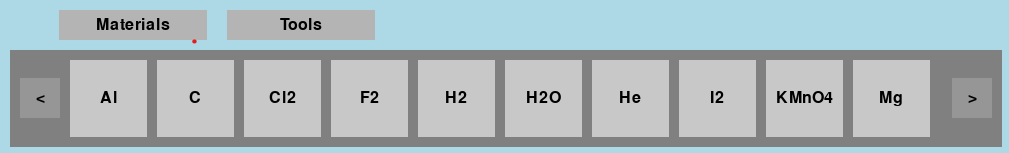
\includegraphics[width=\textwidth]{hotbarM.png}
			\caption{Hotbar materials}
			\label{fig:hotbarM}
		\end{minipage}
		
		\begin{minipage}{0.7\textwidth}
			\centering
			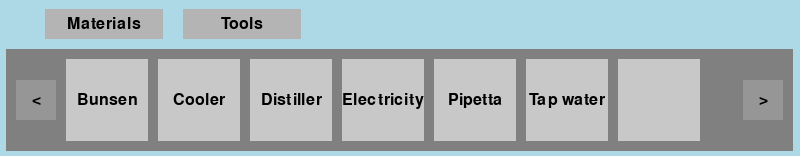
\includegraphics[width=\textwidth]{hotbarT.png}
			\caption{Hotbar tools}
			\label{fig:hotbarT}
		\end{minipage}
		
	\end{figure}
		
	\subsubsection{Trash komponens (trash.py)}
	
	A Trash osztály az objektumok törléséhez szükséges felhasználói felületi komponenst valósítja meg. Alapvető feladatai közé tartozik a törlési zóna megjelenítése és pozícionálása az ablak egy rögzített helyén (jobb felső sarkokban).
	Az egérmozgás figyelése és annak detektálása, hogy mely objektumok vannak a törlési zónában
	Visual feedbacket ad, a kuka sprite-jának frissítésével ha egy adott item a zónába kerül.
	A változást a \ref{fig:trashClosed}. illetve \ref{fig:trashOpen}. ábra szemlélteti.
	
	Ez a komponens szoros kapcsolatban áll az ItemOnBoard-dal, mivel a kuka sprite zónájába kerülő objektumok eltávolításra kerülnek az ItemOnBoard listájából, ezáltal törölve lesznek a játékfelületről is.
	
	\begin{figure}[h]
		\centering
		
		\begin{minipage}{0.4\textwidth}
			\centering
			
\includegraphics[width=\textwidth]{trashClosed.png}
			\caption{Kuka lezárva}
			\label{fig:trashClosed}
		\end{minipage}
		\hfill
		\begin{minipage}{0.45\textwidth}
			\centering
			
\includegraphics[width=\textwidth]{trashOpen.png}
			\caption{Kuka nyitva aktív item-mel a közelében}
			\label{fig:trashOpen}
		\end{minipage}
		
	\end{figure}
	
	
	\subsubsection{SearchSystem modul (searchSystem.py)}
	
	A keresőrendszert implementálja, amely segíti a célzott anyagok előállításában. Funkciói:
	\begin{itemize}
		\item A felhasználó által megadott anyag nevéből indulva az adatbázisban történő keresés
		\item A lehetséges receptek megjelenítése, amelyek az adott anyaghoz vezetnek
	\end{itemize}
	
	\subsubsection{Config modul (config.py)}
	
	Fontos szerepet kap az adatbázis összeköttetés során:
	\begin{itemize}
		\item Az alkalmazás indításakor betölti az összes adatbázis-adatot (anyagok, eszközök, reakciók)
		\item Egy globális adatstruktúrát hoz létre az alkalmazás memóriájában, amely gyors hozzáférést biztosít
		\item Az adatbázis-hibák kezelése (MySQL szerverhez való kapcsolódás sikertelen)
		\item Az adatok frissítésének és szinkronizálásának kezelése
	\end{itemize}
	
	\subsubsection{Tool/materials osztály (/materials.py)}
	
	Az objektumokat definiáló osztályok. A \ref{fig:tools}. ábra a tools osztályt mutatja be.
	
	\lstinputlisting[style=pythonstyle,caption=Tool osztály,label=fig:tools]{tool.py}
	
	\subsubsection{Settings modul (settings.py)}
	
	Az alkalmazás beállításait és konstansait tárja:
	\begin{itemize}
		\item Grafikai beállítások: színek, betűtípusok, margók
		\item Az ablak alapmérete és reszponzivitási szabályai
		\item Konstans értékek: fizikai paraméterek 
		\item A reszponzívitás kiszámításának formulái
	\end{itemize}
	Ez a modul az alkalmazás egészében használt globális konfigurációs adatokat tartalmaz.
	
	\subsection{Adatfolyam és működési logika}
	
	Az alkalmazás működése az alábbi sorrend szerint történik:
	
	\begin{enumerate}
		\item Az alkalmazás indításakor a \texttt{config.py} modul betölti az adatbázisból az összes rendelkezésre álló anyagot, eszközt és kémiai reakciót.
		\item A \texttt{main.py} inicializálja a Pygame-ot és elindítja a fő játékciklust.
		\item Minden frame-ben a rendszer feldolgozza az felhasználói eseményeket: egér eseményeket, mozgásokat és drag-and-drop operációkat.
		\item Az ItemOnBoard komponens frissíti az objektumok pozícióit a felhasználói inputok alapján.
		\item A Reaction modul folyamatosan ellenőrzi az objektumok közötti távolságot, és ha az előfeltételek teljesülnek, reakciókat indít el.
		\item A Pygame végül rendereli a frissített állapotot a képernyőre.
		\item Az Trash és SearchSystem modulok szükség szerint végzik el kiegészítő funkcióikat.
	\end{enumerate}
	
	
	\subsubsection{Pygame keretrendszer integrációja}
	
	A Pygame egy Python alapú grafikus könyvtár, amely SDL (Simple DirectMedia Layer) fölött működik. Az alkalmazásban a Pygame a következő feladatokat végzi:
	
	\begin{itemize}
		\item \textbf{Ablak és megjelenítés:} A Pygame kezeli az alkalmazás ablakát, a felbontást és az átméretezést. Az \texttt{pygame.display} modul kezelő feladata az ablakhoz való rajzolás és az image renderelés.
		
		\item \textbf{Eseménykezelés:} A Pygame az \texttt{pygame.event} modulon keresztül kezeli az összes felhasználói inputot:
		\begin{itemize}
			\item Egérkattintások (\texttt{MOUSEBUTTONDOWN}, \texttt{MOUSEBUTTONUP})
			\item Egérmozgás (\texttt{MOUSEMOTION})
			\item Ablakátméretezés (\texttt{VIDEORESIZE})
			\item Billentyűlenyomások (\texttt{KEYDOWN}, \texttt{KEYUP})
		\end{itemize}
		
		\item \textbf{Grafikus elemek és spritok:} A Pygame a \texttt{pygame.sprite} osztályokkal kezeli az objektumokat.
		
	\end{itemize}
	
	\subsubsection{Adatbázis-kezelés és MySQL integrációja}
	
	Az alkalmazás MySQL adatbázist használ. Az integráció:
	
	\begin{itemize}
		\item \textbf{mysql-connector-python csomag:} Ez a csomag a MySQL szerver és a Python alkalmazás közötti kommunikációt kezelik. Az \texttt{dataBase.py} modul az alábbi műveleteket végzi:
		\begin{itemize}
			\item Kapcsolódás a MySQL szerverhez felhasználónév és jelszó alapján
			\item SQL lekérdezések végrehajtása: SELECT
			\item Hibakezelés: kapcsolódási hibák, lekérdezési hibák, adatkonverziós hibák
		\end{itemize}
		
		
		\item \textbf{Adatbetöltési stratégia:} Az alkalmazás indításakor a \texttt{config.py} modul az összes adatbázis-adatot betölti az alkalmazás memóriájába. Ez a megközelítés:
		\begin{itemize}
			\item Előnye: Gyors adathozzáférés futás közben, mivel az adatok a memóriában vannak
			\item Hátránya: Az alkalmazás memória-igénye növekszik, és az adatbázis módosítása szükséges az alkalmazás újraindításához
		\end{itemize}
	\end{itemize}
	
	\subsubsection{Komponensek közötti kommunikáció}
	
	Az alkalmazás komponensei így kommunikálnak:
	
	\begin{itemize}
		\item \textbf{Main → Config:} Az alkalmazás indításakor a Main osztály meghívja a Config modult az adatok betöltéséhez.
		
		\item \textbf{Main → ItemOnBoard:} A Main osztály kezeli az egéresemények feldolgozását és továbbítja azokat az ItemOnBoard osztálynak.
		
		\item \textbf{ItemOnBoard → Reaction:} Az ItemOnBoard objektumokat hoznak létre és nyomon követik, majd az kombinációk után átadja az információkat a Reaction modulnak.
		
		\item \textbf{Reaction → Config:} A Reaction modul lekérdezi a lehetséges recepteket a Config modulból.
		
		\item \textbf{Hotbar → ItemOnBoard:} A felhasználó által kiválasztott anyagok alapján az ItemOnBoard új objektumokat hoz létre.
		
		\item \textbf{Trash → ItemOnBoard:} Az objektumok törlésének műveletét az ItemOnBoard listájából hajtja végre.
	\end{itemize}
	
	
	\subsubsection{Hibatűrés és hibakezelés}
	
	Az alkalmazás hibalehetőségeit biztosítják:
	
	\begin{itemize}
		\item \textbf{Adatbázis-hiba kezelés:} Ha a MySQL szerver nem érhető el az indítás során, a \texttt{dataBase.py} hibaüzenetet jelenít meg, és az alkalmazás üres listákkal próbál továbblépni.
		
		\item \textbf{Képbetöltési hibák:} Ha egy kép nem található, a Pygame egy alapértelmezett nem a képet jeleníti meg, hanem az item nevét.
		
		\item \textbf{Ablak-átméretezési hibaelkerülés:} A Settings modul biztosítja, hogy az ablak átméretezésekor az összes komponens a helyes pozícióban maradjon.
	\end{itemize}
	
	\subsubsection{Bővíthetőség és fenntarthatóság}
	Az alkalmazás moduláris szerkezete lehetővé teszi az egyszerű bővítést:
	
	\begin{itemize}
		\item \textbf{Új anyagok, reakciók hozzáadása:} Az adatbázisban egy új sor felvétele bármely táblában elegendő az új itemek, reakciók integrálásához.
		
		\item \textbf{Új funkciók:} Az új modulok egyszerűen hozzáadhatók a meglévő szerkezethez.
	\end{itemize}
	
	\section{Adatbázis}
	\subsubsection{Kapcsolatteremtés az adatbázissal}
	
	A backend az alkalmazás szerveroldali logikájáért és az adatok kezeléséért felel. A rendszer az adatbázis-műveletekhez MySQL adatbázist használ, amelyhez a kapcsolat a \texttt{mysql-connector-python} könyvtár segítségével valósul meg.
	
	Az adatkezelési réteg két fő modulra oszlik. A \texttt{config.py} modul felel az alkalmazás indulásakor szükséges alapadatok betöltéséért, ilyenek a reakciók és az itemek adatbázisból történő lekérdezését. Ez biztosítja, hogy a játék logikája dinamikusan, az adatbázis tartalmára alapozva működjön.
	
	A \texttt{database.py} (dataBase.py) modul látja el az adatbázis-hozzáférési réteg szerepét, amely tartalmazza az SQL lekérdezések végrehajtását, valamint az adatok kiolvasását. Ez a réteg elválasztja az adatbázis-kezelési logikát az alkalmazás többi részétől, ezáltal növelve a rendszer modularitását és karbantarthatóságát.
	
	Az adatbázis felépítése lehetővé teszi a játékban használt adatok könnyű bővíthetőségét, mivel az új itemek és reakciók közvetlenül az adatbázis módosításával integrálhatók, a programkód megváltoztatása nélkül.
	
	A backend felelős a játéklogika futtatásáért, beleértve a reakciók ellenőrzését és az objektumok közötti interakciók kezelését. A rendszer folyamatosan figyeli a játékterületen lévő elemek közötti távolságot, és meghatározott feltételek teljesülése esetén reakciókat indít el.
	
	A háttérfolyamatok eseményvezérelt módon működnek, amelyet a PyGame fő ciklusa (game loop) hajt végre. Ez biztosítja, hogy a játék állapota minden frame-ben frissüljön, miközben az adatkezelés és a logikai műveletek elkülönítve, mégis szinkronban történnek.
	\subsubsection{Adatbázis-struktúra:}
	
	Az alkalmazás három táblát használ, amelyeket a \ref{fig:database}. ábra prezentál egy dbdiagrammal\cite{dbDiagram}:
	\begin{itemize}
		\item \textbf{reactions:} A kémiai reakciókat definiálja (item1,item2,result,equation,type). Item1 és item2 mező a reakcióhoz használt bemeneti elemeket tárolja, amelyekkel létrejön egy adott típusú eredmény(result). A folyamat képletét az equation tárolja el.
		\item \textbf{tools:} Az eszközök nevét tartalmazza. 
		\item \textbf{materials tábla:} A kémiai anyagok nevét tárolja.
		
	\end{itemize}
	
	\begin{figure}[h]
		\centering
		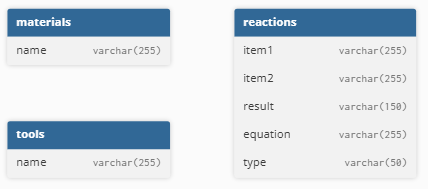
\includegraphics[width=0.7\textwidth]{dataBaseStructure.png}
		\caption{Adatbázis felépítése}
		\label{fig:database}
	\end{figure}
	Az adatbázis kapcsolatokat nem tartalmaz, mivel a további feldolgozást a program végzi.
	
	
	\section{Frontend}
	
	A frontend megvalósítása a PyGame könyvtár felhasználásával történt, amely egy Python alapú, 2D grafikus alkalmazások fejlesztésére alkalmas keretrendszer. A rendszer főbb feladatai közé tartozik a felhasználói interakciók kezelése, a grafikus elemek megjelenítése, valamint a játéklogika vizuális visszacsatolásának biztosítása.
	
	Az alkalmazás támogatja a drag-and-drop mechanizmust, amely lehetővé teszi az objektumok interaktív mozgatását a játéktéren belül. Emellett a felület reszponzív kialakítással rendelkezik, amely biztosítja, hogy az ablakméret változásakor a grafikus komponensek elrendezése és méretezése dinamikusan alkalmazkodjon az aktuális képernyőmérethez.
	
	A reszponzív működés alapját egy központi layout-számítási mechanizmus képezi, amely az aktuális ablakméretből (szélesség és magasság) származtatja a felhasználói felület fő elemeinek, például a játéktérnek és a hotbar komponenseknek méreteit. Az átméretezési események kezelése során a rendszer újraszámolja a vizuális elemek pozícióit, így biztosítva az arányos megjelenítést különböző felbontások esetén is.
	
	A vizuális visszajelzések között tooltip-ek, valamint reakcióláncok (history chain) megjelenítése szerepel, amelyek segítik a felhasználót a játékbeli interakciók követésében és értelmezésében.
	
	\subsubsection{Képek}
	
	A játékban használt grafikai elemeket a Piskel\cite{Piskel} online szerkesztő segítségével készültek. Az sprite-ok PNG formátumú, átlátszó hátterű képek, amelyek könnyedén felhasználhatóak a PyGame segítségével.
	
	Ilyen sprite a \ref{fig:Pipetta}. ábrán látható pipetta eszköz is amely víz felvétele után a \ref{fig:Pipetta(H2O)}. ábra látható már anyagként.
	
	\begin{figure}[h]
		\centering
		
		\begin{minipage}{0.45\textwidth}
			\centering
			
\includegraphics[width=\textwidth]{Pipetta.png}
			\caption{Pipetta sprite}
			\label{fig:Pipetta}
		\end{minipage}
		\hfill
		\begin{minipage}{0.45\textwidth}
			\centering
			
\includegraphics[width=\textwidth]{Pipetta(H2O).png}
			\caption{Pipetta(H2O) sprite}
			\label{fig:Pipetta(H2O)}
		\end{minipage}
		
	\end{figure}
	
	\chapter{Futtatás}
	
	A program Python 3.10 környezetben készült. A futtatáshoz MySQL szerverre, valamint a \texttt{pygame} és \texttt{mysql-connector-python} Python-csomagokra van szükség. A tesztek futtatásához a \texttt{pytest} csomag is szükséges.
	
	A programot a projekt gyökérkönyvtárából kell indítani, mivel az alkalmazás a képfájlokat relatív útvonalakon keresztül tölti be az \texttt{img/materials} és \texttt{img/tools} mappákból.
	
	\section{Környezet előkészítése (Windows PowerShell)}
	
	A virtuális környezet létrehozása és a függőségek telepítése az alábbi parancsokkal történik:
	
	\begin{verbatim}
		cd szakdolgozat-main
		python -m venv venv
		.\venv\Scripts\Activate.ps1
		python -m pip install pygame mysql-connector-python pytest
	\end{verbatim}
	
	Amennyiben a projekt tartalmaz \texttt{requirements.txt} fájlt, a csomagok telepítése a következő paranccsal végezhető el:
	
	\begin{verbatim}
		python -m pip install -r requirements.txt
	\end{verbatim}
	
	\section{Adatbázis}
	
	A program alapértelmezés szerint a localhoston futó MySQL szerverhez kapcsolódik \texttt{root} felhasználóval, üres jelszóval, a \texttt{labor} nevű adatbázishoz. Ettől eltérő beállítás esetén a \texttt{src/dataBase.py} fájlban található kapcsolódási adatokat módosítani kell.
	
	Az adatbázis három fő táblát használ: \texttt{materials}, \texttt{tools} és \texttt{reactions}. A \texttt{materials} és \texttt{tools} táblák az alkalmazásban megjeleníthető anyagokat és eszközöket tartalmazzák, míg a \texttt{reactions} tábla az egyes reakciók bemeneti elemeit, eredményét és egyenletét tárolja.
	
	Az adatbázis inicializálásához a mellékelt \texttt{database.sql} fájl futtatása szükséges.
	
	\section{Program indítása}
	
	Az alkalmazás indítása:
	
	\begin{verbatim}
		python src/main.py
	\end{verbatim}
	
	Sikeres indítás után megjelenik a \textit{Labor} című Pygame ablak. Az alsó hotbarban az adatbázisból betöltött anyagok és eszközök jelennek meg. Az elemek a játéktérre húzhatók, kompatibilis anyagok esetén pedig új reakciótermék jön létre.
	
	\section{Hibaelhárítás}
	
	Ha a MySQL szerver nem fut, vagy a \texttt{labor} adatbázis nem érhető el, a program hibaüzenetet ír ki, és az adatbázisból betöltött listák üresek maradnak. Ebben az esetben ellenőrizni kell a MySQL szolgáltatás állapotát, az adatbázis nevét és a kapcsolódási adatokat.
	
	\chapter{Tesztelés}
	
	\section{Manuális tesztelés}
	\begin{table}[ht!]
		\centering
		\footnotesize
		\begin{tabular}{|>{\centering}m{4.5cm}|>{\centering}m{3cm}|>{\centering\arraybackslash}m{7cm}|}
			\hline
			\textbf{Funkció} & \textbf{Leírás} & \textbf{Opciók/Példák} \\
			\hline
			Hotbar váltás & Sikeres & Gombok megfelelően váltanak hotbar-t \\
			\hline
			Material helyezése a játékfelületre & Sikeres & A material megjelent a a játékfelületen \\
			\hline
			Tool helyezése a játékfelületre & Sikeres & A tool megjelent a a játékfelületen \\
			\hline
			Adatbázis betöltése & Sikeres & Sikeresen betöltöttek az adatok \\
			\hline
			Két material reakciója & Sikeres & Új material jött létre, sikeres \\
			\hline
			Material és tool reakciója & Sikeres & Sikeres reakció \\
			\hline
			Kuka megjelenése & Sikeres & Kuka jó helyen jelent meg \\
			\hline
			Kuka reszponzívan tartja a helyét & Sikeres & Kuka jó helyen jelent meg \\
			\hline
			Kuka sprite váltása ha adott item van a közelében & Sikeres & A kuka megfelelően vált sprite-ot \\
			\hline
			Keresés jó eredményeket ad ki & Sikertelen (javítva) & A keresés nem ad ki nemlétező eredményeket \\
			\hline
			Az itemek pozícionálása ablakméret váltáskor & Sikeres & Az itemek megfelelő helyen vannak ablakméret váltáskor \\
			\hline
			A hotbár reszponzív & Sikertelen (javítva) & Nagyításkor eltűnik - rossz pozícionálás, javítva\\
			\hline
			Itemek adatainak kiíratása & Sikeres & Megfelel adatok jelennek meg az itemek alatt \\
			\hline
			Hotbar léptetése a materials itemeknél & Sikeres & Összes item megtekinthető \\
			\hline
			Sprite-ok megjelnése & Sikeres & A sprite-ok megfelelően jelennek meg \\
			\hline
		\end{tabular}
		\caption{Manuális teszt jegyzőkönyv}
		\label{MTeszt-jegyzokonyv}
	\end{table}
	
	\section{Integrációs tesztelési forgatókönyvek}
	
	\begin{table}[ht!]
		\centering
		\footnotesize
		\begin{tabular}{|p{4cm}|p{4cm}|p{4cm}|p{3.5cm}|}
			\hline
			\textbf{Teszt neve} & \textbf{Bemenet} & \textbf{Folyamat} & \textbf{Elvárt kimenet} \\
			\hline
			H2O reakció integrációs teszt
			& H2 + O2 elhelyezése a játéktéren egymás közelében
			& Reaction.check() felismeri a párost, can\_react(H2, O2) igaz, adatbázisból lekéri a reakciót
			& Új item: H2O megjelenik, H2 és O2 törlődik a pályáról \\
			
			\hline
			
			Nem definiált reakció kezelése
			& Na + Cl elhelyezése egymás közelében
			& Reaction.check() fut, can\_react(Na, Cl) nem talál adatbázisbeli egyezést
			& Nincs változás a játékállapotban, itemek maradnak \\
			
			\hline
			
		\end{tabular}
		\caption{Integrációs tesztelési forgatókönyvek}
		\label{tab:ITest}
	\end{table}
	
	
	\section{Automatikus tesztelés}
	\begin{table}[ht!]
		\centering
		\footnotesize
		\begin{tabular}{|>{\centering}m{4.5cm}|>{\centering}m{3cm}|>{\centering\arraybackslash}m{7cm}|}
			\hline
			\textbf{Funkció} & \textbf{Leírás} & \textbf{Opciók/Példák} \\
			\hline
			get\_recipe() függvény működése  H2O-ra, NaCl-ra CO-ra,CO2-ra, & Sikeres & Megfelelően visszadja a kiinduló alapanyagokat \\
			\hline
			can\_react() függvény működése H2+O2-re & Sikeres & Sikeres reakciótalálat \\
			\hline
			can\_react() függvény negatív teszteset Na+Cl-re & Sikeres & Sikeres, nem talált reakciót \\
			\hline
			check() függvény tesztelése & Sikeres & Az anyag létrejött \\
			\hline
			check() függvény tesztelése több kimenetre & Sikeres & Reakció után megfelelő számú anyag spawnolt \\
			\hline
			reaction() függvény tesztelése, használt itemek törlése & Sikeres & Reakció után az itemek törlődnek \\
			\hline
			delete\_item() függvény tesztelése & Sikeres & Item sikeresen törlődik\\
			\hline
			trash\_hover() függvény működése & Sikeres & Megfelelően működik\\
			\hline
			trash\_draw() függvény működése & Sikeres & Megfelelően kirajzolódik\\
			\hline
		\end{tabular}
		\caption{Automatikus tesztelési jegyzőkönyv}
		\label{ATeszt-jegyzokonyv}
	\end{table}
	Az automatikus tesztek megvalósításához a Python beépített unittest.mock\cite{unittest_mock} könyvtárát, valamint a pytest\cite{pytest} tesztelési keretrendszert alkalmaztam. A unittest.mock lehetővé teszi helyettesítő objektumok létrehozását a valós függőségek kiváltására tesztkörnyezetben.
	
	A mock objektumok segítségével a függőségek viselkedése előre definiálható, valamint ellenőrizhető, hogy egy adott metódus milyen paraméterekkel és hányszor került meghívásra. Ez növeli a tesztek izoláltságát, megbízhatóságát és olvashatóságát, míg a pytest egyszerű és skálázható tesztfuttatást biztosít.
	
	\chapter{Összegzés}
	
	A fejlesztés során kiemelt szerepet kapott a felhasználói élmény kialakítása. A drag-and-drop mechanizmus, a reszponzív felület, valamint a vizuális visszajelzések azt a célt szolgálták, hogy a tanulási folyamat minél intuitívabb és motiválóbb legyen.
	
	A tesztelési fázis során végzett megfigyelések alapján a felhasználók rövid időn belül képesek voltak elsajátítani az alkalmazás alapvető használatát, és a vizuális elemek segítették a kémiai összefüggések értelmezését.
	
	A rendszer jelenlegi formájában stabilan működik, azonban több irányban is továbbfejleszthető, például hang- és vizuális effektek, reakcióanimációk, valamint egy részletesebb oktatási modul bevezetésével.
	
	A rendszer jelenlegi korlátja a reakciókezelés implementációja. A \texttt{src/reaction.py} modulban alkalmazott \texttt{frozenset} alapú megközelítés egyszerű és hatékony az alap bináris reakciók kezelésére, azonban nem támogatja megfelelően az azonos reagenseket.. Ennek következtében a modell csak egyszerű, kétkomponensű reakciók esetén megbízható.
	
	További korlát, hogy az alkalmazás teljes adatbázis-betöltésre épül, így nagy mennyiségű adat esetén memóriahasználati problémák jelentkezhetnek, valamint az adatváltozások csak újraindítás után érvényesülnek.
	
	Összességében a létrehozott alkalmazás technikai szempontból sikeresen megvalósult, és potenciálisan alkalmas lehet az oktatási folyamat támogatására, azonban pedagógiai hatékonyságának objektív értékeléséhez további felhasználói vizsgálatok szükségesek.
	
	\begin{thebibliography}{2}
		\addcontentsline{toc}{chapter}{\bibname}
		\bibitem{Piskel}
		\textsc{Piskel}: \emph{Online pixel art és sprite szerkesztő}, https://www.piskelapp.com/ (Letöltés: 2026.04.21.)
		
		\bibitem{Python}
		\textsc{Python Software Foundation}: \emph{Python 3 hivatalos dokumentáció}, https://docs.python.org/3/ (Letöltés: 2026.04.21.)
		
		\bibitem{PyGame}
		\textsc{Pygame}: \emph{Hivatalos Pygame dokumentáció}, https://www.pygame.org/docs/ (Letöltés: 2026.04.21.)
		
		\bibitem{PyCharm}
		\textsc{JetBrains}: \emph{PyCharm Getting Started – Hivatalos bevezető és útmutató}, https://www.jetbrains.com/help/pycharm/getting-started.html (Letöltés: 2026.04.21.)
		
		\bibitem{Apache}
		\textsc{Apache Friends}: \emph{XAMPP hivatalos letöltési és dokumentációs oldal}, https://www.apachefriends.org/ (Letöltés: 2026.04.21.)
		
		\bibitem{phpMyAdmin}
		\textsc{phpMyAdmin}: \emph{Hivatalos phpMyAdmin dokumentáció és letöltési oldal}, https://www.phpmyadmin.net/ (Letöltés: 2026.04.21.)
		
		\bibitem{GitHub}
		\textsc{GitHub}: \emph{GitHub témák és dokumentációs gyűjtemények}, https://github.com/topics/documentation (Letöltés: 2026.04.21.)
		
		\bibitem{VisualStudioCode}
		\textsc{Microsoft}: \emph{Visual Studio Code hivatalos dokumentáció}, https://code.visualstudio.com/docs (Letöltés: 2026.04.21.)
		
		\bibitem{Git}
		\textsc{Git}: \emph{Hivatalos Git dokumentáció}, https://git-scm.com/docs (Letöltés: 2026.04.21.)
		
		\bibitem{dbDiagram}
		\textsc{dbdiagram.io}: \emph{Hivatalos dokumentáció – adatbázis diagramok és DBML leírás}, https://docs.dbdiagram.io/ (Letöltés: 2026.04.21.)
		
		\bibitem{Oracle}
		\textsc{Oracle}: \emph{MySQL Connector/Python hivatalos dokumentáció}, https://dev.mysql.com/doc/connector-python/en/ (Letöltés: 2026.04.21.)
		
		\bibitem{C++}
		\textsc{DevDocs}: \emph{C++ referencia dokumentáció (C/C++ API és standard library leírások gyűjteménye)}, https://devdocs.io/cpp/ (Letöltés: 2026.04.21.)
		
		\bibitem{C-Sharp}
		\textsc{Microsoft Learn}: \emph{C\# hivatalos dokumentáció és útmutató (.NET platform)}, https://learn.microsoft.com/en-us/dotnet/csharp/ (Letöltés: 2026.04.21.)
		
		\bibitem{Java}
		\textsc{Oracle}: \emph{Java Platform, Standard Edition (Java SE) hivatalos dokumentáció}, https://docs.oracle.com/en/java/ (Letöltés: 2026.04.21.)
		
		\bibitem{SQL}
		\textsc{W3Schools}: \emph{SQL Tutorial és referenciaanyag (SQL nyelv alapjai, lekérdezések és példák)}, https://www.w3schools.com/sql/ (Letöltés: 2026.04.21.)
		
		\bibitem{Kombination}
		\textsc{ITU Online}: \emph{What Is Python Pygame?}, https://www.ituonline.com/tech-definitions/what-is-python-pygame/ (Letöltés: 2026.04.21.)
		
		
		\bibitem{PyGame2}
		\textsc{Dr. M. K. Jayanthi Kannan}: \emph{Introduction to Pygame and Game Development using Python Pygame}, ResearchGate, https://www.researchgate.net/publication/377064275\_Introduction\_to\_Pygame\\\_and\_Game\_Development\_using\_Python\_Pygame\_by\_Dr\_MK\_Jayanthi\\\_Kannan (Letöltés: 2026.04.21.)
		
		\bibitem{SDL}
		\textsc{Simple DirectMedia Layer (SDL)}: \emph{Official SDL homepage}, https://www.libsdl.org/ (Letöltés: 2026.04.21.)
		
		\bibitem{unittest_mock}
		\textsc{Python Software Foundation}: \emph{The unittest.mock library — mock object library for testing in Python}, https://docs.python.org/3/library/unittest.mock.html (Letöltés: 2026.04.22.)
		
		\bibitem{pytest}
		\textsc{pytest Project}: \emph{pytest: helps you write better programs – official documentation}, https://docs.pytest.org/en/stable/ (Letöltés: 2026.04.22.)
		
	\end{thebibliography}
	
	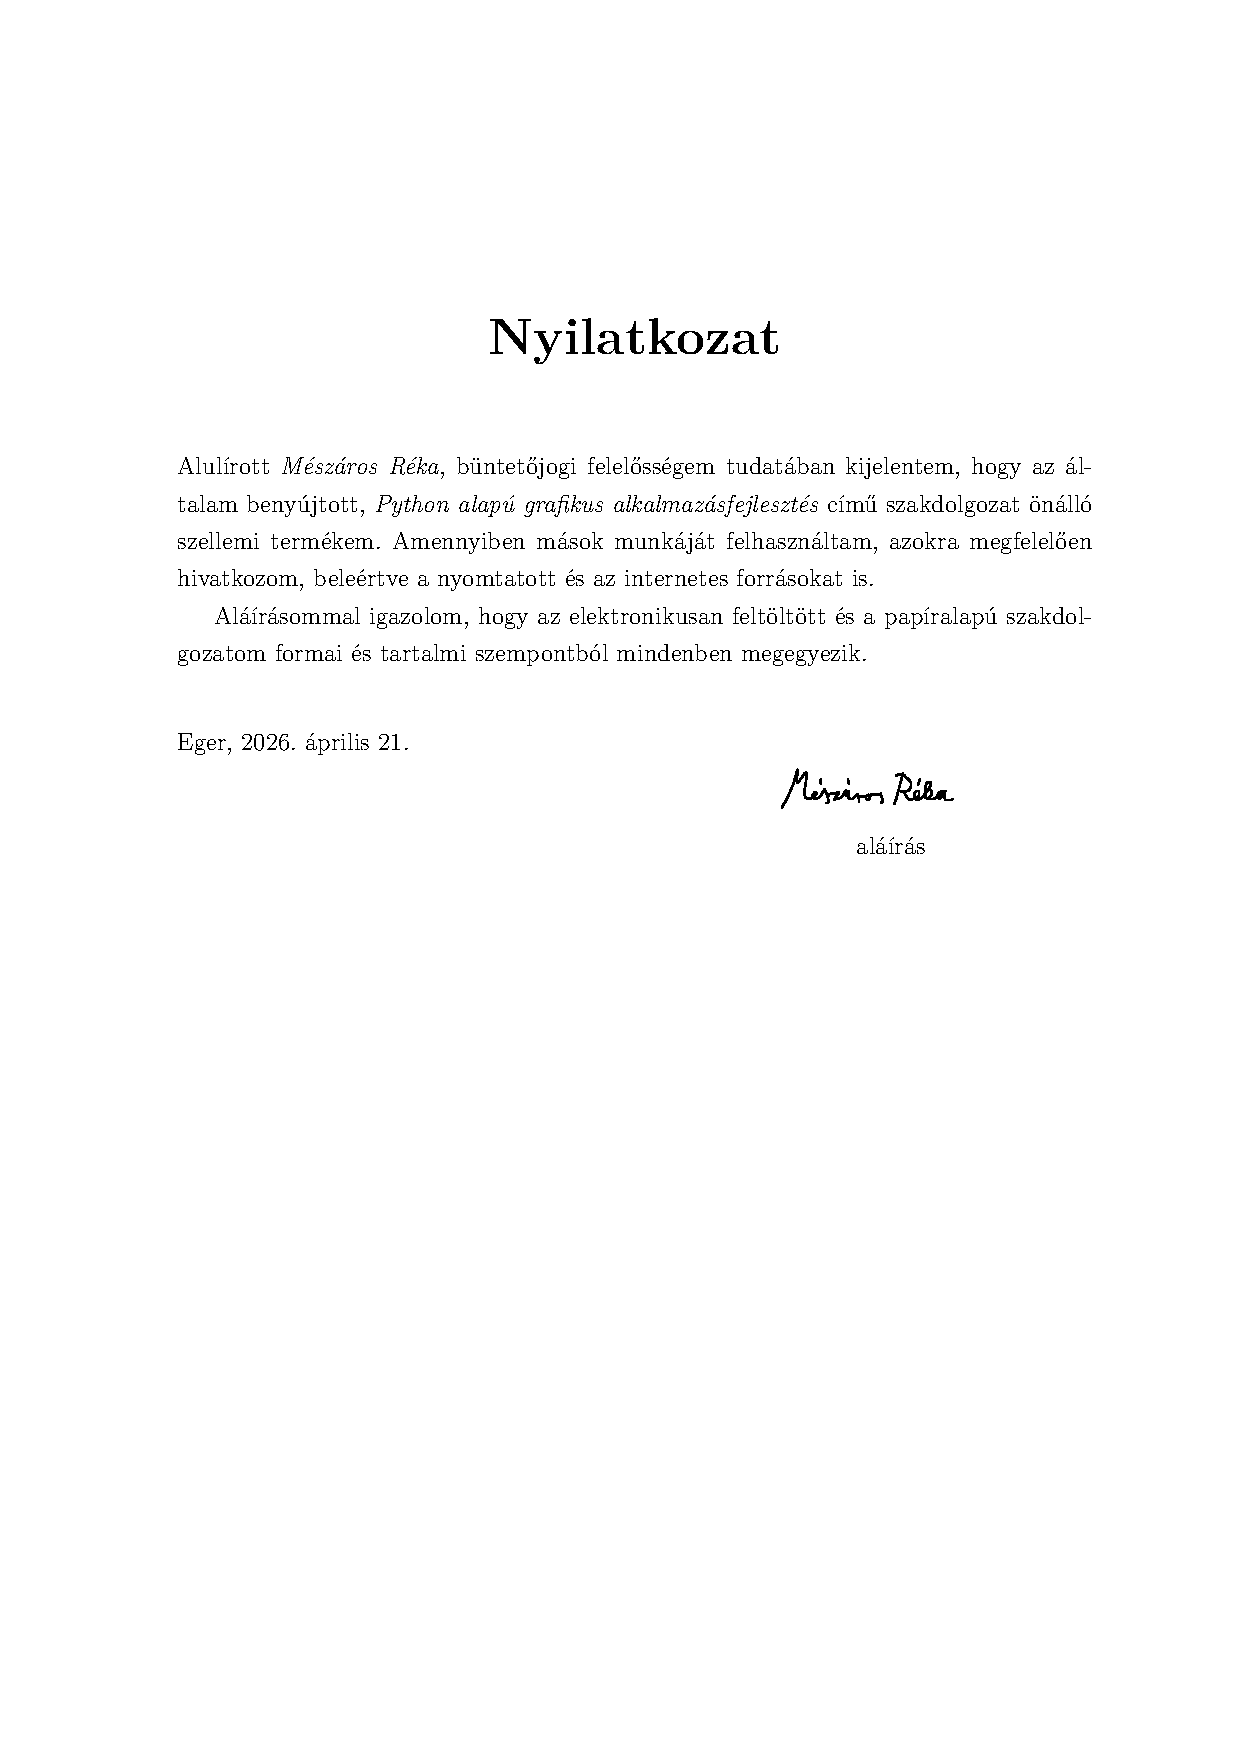
\includepdf{Nyilatkozat.pdf} 
	
\end{document}
